\documentclass[tikz,border=10pt]{standalone}
\usepackage{pgfplots}
\pgfplotsset{compat=1.18}
\usepackage{amsmath,amssymb,bm}
\definecolor{darkbg}{HTML}{ffffff}
\definecolor{lightfg}{HTML}{333333}
\definecolor{accent}{HTML}{2d7d46}
\definecolor{accent2}{HTML}{2d6d7d}
\definecolor{mutedcol}{HTML}{888888}
\definecolor{bordercol}{HTML}{cccccc}
\definecolor{redcol}{HTML}{cc3333}
\definecolor{bluecol}{HTML}{3355bb}
\color{lightfg}

\usetikzlibrary{arrows.meta}

\begin{document}
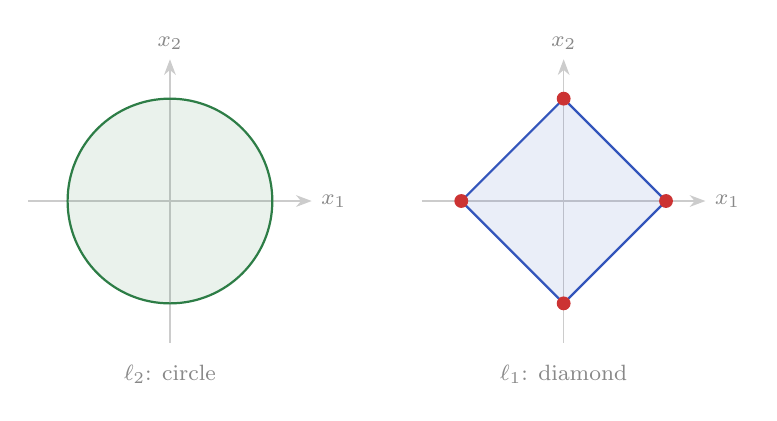
\begin{tikzpicture}

% === LEFT PANEL: L2 unit ball (circle) ===
\begin{scope}[shift={(0,0)}]
  \draw[bordercol, thin, -{Stealth[length=2mm]}] (-1.8,0) -- (1.8,0)
    node[right, mutedcol, font=\footnotesize] {$x_1$};
  \draw[bordercol, thin, -{Stealth[length=2mm]}] (0,-1.8) -- (0,1.8)
    node[above, mutedcol, font=\footnotesize] {$x_2$};

  \fill[accent, opacity=0.1] (0,0) circle (1.3);
  \draw[accent, thick] (0,0) circle (1.3);

  \node[mutedcol, font=\footnotesize] at (0,-2.2) {$\ell_2$: circle};
\end{scope}

% === RIGHT PANEL: L1 unit ball (diamond) ===
\begin{scope}[shift={(5,0)}]
  \draw[bordercol, thin, -{Stealth[length=2mm]}] (-1.8,0) -- (1.8,0)
    node[right, mutedcol, font=\footnotesize] {$x_1$};
  \draw[bordercol, thin, -{Stealth[length=2mm]}] (0,-1.8) -- (0,1.8)
    node[above, mutedcol, font=\footnotesize] {$x_2$};

  \fill[bluecol, opacity=0.1] (1.3,0) -- (0,1.3) -- (-1.3,0) -- (0,-1.3) -- cycle;
  \draw[bluecol, thick] (1.3,0) -- (0,1.3) -- (-1.3,0) -- (0,-1.3) -- cycle;

  \fill[redcol] (1.3,0) circle (2.5pt);
  \fill[redcol] (-1.3,0) circle (2.5pt);
  \fill[redcol] (0,1.3) circle (2.5pt);
  \fill[redcol] (0,-1.3) circle (2.5pt);

  \node[mutedcol, font=\footnotesize] at (0,-2.2) {$\ell_1$: diamond};
\end{scope}

\end{tikzpicture}
\end{document}
